\documentclass[a4paper, 11pt, oneside]{book} % A4 paper size, default 11pt font size and oneside for equal margins

\newcommand{\plogo}{\fbox{$\mathcal{PL}$}} % Generic dummy publisher logo

\usepackage[utf8]{inputenc} % Required for inputting international characters
\usepackage[T1]{fontenc} % Output font encoding for international characters
\usepackage{fouriernc} % Use the New Century Schoolbook font
\usepackage{graphicx}
\graphicspath{ {./images/} }

%----------------------------------------------------------------------------------------
%	TITLE PAGE
%----------------------------------------------------------------------------------------

\begin{document} 

\begin{titlepage} % Suppresses headers and footers on the title page

	\centering % Centre everything on the title page
	
	\scshape % Use small caps for all text on the title page
	
	\vspace*{\baselineskip} % White space at the top of the page
	
	%------------------------------------------------
	%	Title
	%------------------------------------------------
	
	\rule{\textwidth}{1.6pt}\vspace*{-\baselineskip}\vspace*{2pt} % Thick horizontal rule
	\rule{\textwidth}{0.4pt} % Thin horizontal rule
	
	\vspace{0.75\baselineskip} % Whitespace above the title
	
	{\LARGE Calculus\\ 2\\} % Title
	
	\vspace{0.75\baselineskip} % Whitespace below the title
	
	\rule{\textwidth}{0.4pt}\vspace*{-\baselineskip}\vspace{3.2pt} % Thin horizontal rule
	\rule{\textwidth}{1.6pt} % Thick horizontal rule
	
	\vspace{2\baselineskip} % Whitespace after the title block
	
	%------------------------------------------------
	%	Subtitle
	%------------------------------------------------
	
	Kinetic Energy % Subtitle or further description
	
	\vspace*{3\baselineskip} % Whitespace under the subtitle
	
	%------------------------------------------------
	%	Editor(s)
	%------------------------------------------------
	
	Created By
	
	\vspace{0.5\baselineskip} % Whitespace before the editors
	
	{\scshape\Large Ben Cordova \\ Colin hay \\ Harry Margalotti \\} % Editor list
	
	\vspace{1.0\baselineskip} % Whitespace below the editor list
	
	
	\textit{Ithaca College \\} % Editor affiliation
	
	\vfill % Whitespace between editor names and publisher logo
	
	2019 % Publication year
	

\end{titlepage}
%----------------------------------------------------------------------------------------
\pagebreak{}
\centering % Centre everything on the title page
{\LARGE Intro\\} % Title
\vspace{0.5\baselineskip} % Whitespace before the editors
In this paper, we will be exploring the real world applications of calculating linear and angular velocities in different scenarios. We will model, a record, a helicopter, and the earth throughout the paper, in our equations.
\vspace{1.0\baselineskip} % Whitespace before the editors

{\LARGE Why cant we apply the kinetic energy formula directly? \\} % Title
\vspace{0.5\baselineskip} % Whitespace before the editors
We cannot use the formula for kinetic energy to directly estimate our models. This is because the formula for kinetic energy is linear, yet our models deal with angular velocity. In each model, the record, the helicopter blade, and the Earth, we are measuring the kinetic energy of an object about its axis. This requires us to use the slice and add modeling approach for integrals. By calculating the mass and velocity of individual slices we are able to estimate the total kinetic energy of an object.

\vspace{1.0\baselineskip} % Whitespace before the editors

{\LARGE The Record \\} % Title
\vspace{0.5\baselineskip} % Whitespace before the editors
To calculate the kinetic energy of a record as it plays on a record player we must slice the model into smaller parts. We have decided to think of the record as a collection of circular strips, radiating out from the center. This is convenient because our formula for angular velocity requires the object to be circular. By finding the angular velocity and mass of our slices, we are able to estimate the kinetic energy of the entire object. 
To start we will estimate the area of the record using an integral. By using the circumference of a circle, and thinking of our circular slice as a rectangle, we are able to derive the following integral.
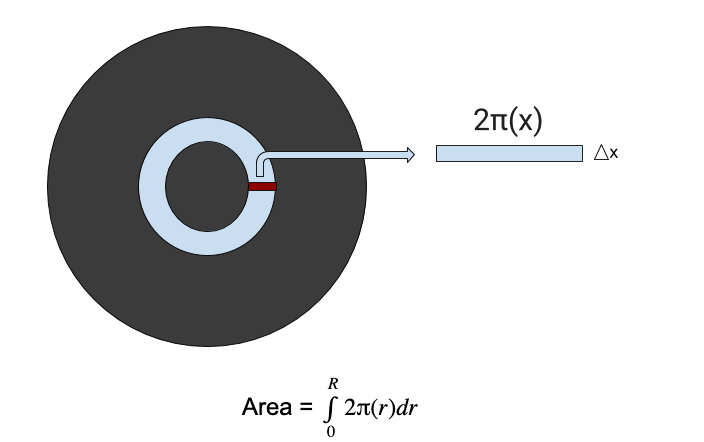
\includegraphics[scale=0.38]{record1}\\
Now that we have an integral to represent the area of the record, we can build upon it to estimate the mass. The formula for mass is: \newline
{\large {Mass = V * d\\} }
{\large {V =  Area * h\\} }
To estimate the mass we must first find the volume. We are going to assume that our record has constant height and density. By multiplying our area by our height we can compute volume, and multiplying that by our density leaves us with an estimate for mass. \newline
{\large {$$\int_{0}^{R} hd2\pi(r)dr$$\\} }
We must again add to this integral. We are currently estimating the mass of the record and our next step is to estimate the linear velocity. The formula for linear velocity is: \newline
\newline
{\large {Linear Velocity = $\omega$ r \\} } 
\vspace{0.5\baselineskip} % Whitespace before the editors
To calculate linear velocity of each slice  we must multiply angular velocity $\omega$ by the radius (r). \newline
\newline
{\large {Linear Velocity = $\int_{0}^{R} \omega r dr$\\} }
\vspace{0.5\baselineskip} % Whitespace before the editors
Now that we have found integrals for mass and linear velocity we can apply our formula for kinetic energy. \newline
\newline
{\large {K = $\frac{1}{2}mv^2$ \\} }
\vspace{0.5\baselineskip} % Whitespace before the editors
{\large {K = $\int_{0}{R} \frac{1}{2}(hd2\pi(r))(\omega r)^2 dr$ \\} }
\vspace{0.5\baselineskip} % Whitespace before the editors
This integral should calculate the total kinetic energy of the record, evaluated for each slice. We can further simplify our integral by pulling out constants.\\
\vspace{0.5\baselineskip} % Whitespace before the editors
{\large {K = $hd\pi \omega^2$ $\int_{0}^{R} r^3 dr$ \\} }
\vspace{0.5\baselineskip} % Whitespace before the editors
Finally we can integrate this equation to further simplify. \\
\vspace{0.5\baselineskip} % Whitespace before the editors
{\large {K = $hd\pi \omega^2(\frac{R^4}{4})$\\} }
Looking at the wikipedia page for LP record we see that a common 12 inch LP Record has the following characteristics.\\
\vspace{0.5\baselineskip} % Whitespace before the editors
\begin{table}[!h]
\centering
\begin{tabular}{lllll}
Radius & Height & Density & Angular Velocity &  \\
0.1524 m (6 in) & 0.001 m (1 mm) & $\frac{1350kg}{m^3}$($\frac{1.35 g}{cm^3}$) & 3.49065 $\frac{rad}{s}$ (33$\frac{1}{3}$rpm) &  \\
 &  &  &  &  \\
 &  &  &  & 
\end{tabular}
\end{table}
\textit{`many of the thinnest [LP Records] (0.9 to 1.0 mm) were the most uniform in thickness and some of the best sounding`} 
-tketcham \\
We have chosen to go with 1 mm as our record thickness to make our calculations easier. We also convert this to meters to match the units of the kinetic energy formula.\\
\vspace{0.5\baselineskip} % Whitespace before the editors
$1mm$ * $\frac{1m}{1000mm}$ = $0.001m$\\
\vspace{0.5\baselineskip} % Whitespace before the editors
We then found that LP Records were commonly made out of polyvinyl chloride which typically has a density of 1.35 g/c$m^3$. Again we convert this to kg/$m^3$ to match the units of kinetic energy.\\
\vspace{0.5\baselineskip} % Whitespace before the editors
($\frac{1.35g}{cm^3}) * (\frac{1kg}{1000g}) * (\frac{1000000cm^3}{1m^3}) = \frac{1350kg}{m^3}$\\
\vspace{0.5\baselineskip} % Whitespace before the editors
Finally we found from the LP Record wikipedia page that 12 inch records typically spun at 33 $\frac{1}{3}$ rpms. We then converted this to radians per second to match the units of kinetic energy. \\
\vspace{0.5\baselineskip} % Whitespace before the editors
(33.3333 $\frac{rev}{min}$) * ($\frac{1min}{60s}$) * (2$\pi \frac{rad}{1rev}$) = 3.49065 $\frac{rad}{s}$\\
\vspace{0.5\baselineskip} % Whitespace before the editors
To confirm our previous work we are going to check the units of our formula given these values. Kinetic energy is typically measured in Joules:\\
\vspace{0.5\baselineskip} % Whitespace before the editors
\large{$J = \frac{(1kg * m^2)}{s^2}$}\\
\vspace{0.5\baselineskip} % Whitespace before the editors
The units for our formula are: \\
\vspace{0.5\baselineskip} % Whitespace before the editors
\large{$m$ * ($\frac{kg}{m^3}$) * ($\frac{rad}{s})^2$ * $m^4$\\
\vspace{0.5\baselineskip} % Whitespace before the editors
\large{$kg * \frac{m^2}{s^2}$}\\
\vspace{0.5\baselineskip} % Whitespace before the editors
As you can see the units for our formula model the units for Jules. This gives us confidence that the formula we derived for kinetic energy is accurate. Now we can plug assumed values into our formula to start estimating the kinetic energy of a record. \\
\vspace{0.5\baselineskip} % Whitespace before the editors
$\frac{((0.001)(1350)\pi(3.49065^2)(0.1524^4)}{4}$\\
\vspace{0.5\baselineskip} % Whitespace before the editors
\large{=}\\
\vspace{0.5\baselineskip} % Whitespace before the editors
$0.00696909088(\frac{kg*m^2}{s^2})$\\
\vspace{0.5\baselineskip} % Whitespace before the editors
$K = 0.00696909088J$\\
This is our estimate for the kinetic energy of a record rotating at 33 $\frac{1}{3}$  rpms, with a diameter of 12 inches, height of 1 mm, and density of $\frac{1.35g}{cm^3}$ . To check our answer, we have found the average mass of a record of this size to range from 90g to 240g. Therefore we have decided to use 0.15kg (150g), which is the midpoint between the two values. We will plug this into a new integral we have derived that substitutes our calculation for mass with this specific value. This will allow us to compare our estimates that used volume and density with the average mass of a record.\\
\vspace{0.5\baselineskip} % Whitespace before the editors
$K = \int_{0}^{R} (\frac{1}{2})(m)(\omega r)^2dr$\\
\vspace{0.5\baselineskip} % Whitespace before the editors
$K = (\frac{1}{6})m\omega^2R^3$\\
\vspace{0.5\baselineskip} % Whitespace before the editors
$K =  (\frac{1}{6})(0.15)(3.49065)^2(0.1524)^3$\\
\vspace{0.5\baselineskip} % Whitespace before the editors
\large{=}\\
\vspace{0.5\baselineskip} % Whitespace before the editors
$0.00107822033(\frac{(kg * m^2)}{s^2})$\\
\vspace{0.5\baselineskip} % Whitespace before the editors
$K = 0.00107822033 J$\\
\vspace{0.5\baselineskip} % Whitespace before the editors
To help confirm our answer we are going to calculate what our formula calculated the mass of the record to be given the height, density, and radius. If this value falls between the average mass of a record, 90g to 240g, then we can be more confident in our result.\\
\vspace{0.5\baselineskip} % Whitespace before the editors
$Mass =  \int_{0}^{R} hd2\pi r dr$\\
\vspace{0.5\baselineskip} % Whitespace before the editors
$Mass = hd\pi r^2$\\
\vspace{0.5\baselineskip} % Whitespace before the editors
$Mass = 0.001 * 1350 * \pi * 0.1524^2$\\
\vspace{0.5\baselineskip} % Whitespace before the editors
$Mass = 0.0985kg = 98.5g$\\
\vspace{0.5\baselineskip} % Whitespace before the editors
This calculation shows that our formula estimated the mass of the record to be 98.5 g which is between the average masses of 90g and 240g. This estimate still certainly has many flaws. We are unsure if LP Records are made completely out of polyvinyl chloride. We also did not account for the fact that a record would not have a constant density because of the grooves. We still have faith in our formula because the units correctly work out to give us the units for Joules, however our assumptions most likely introduced a significant amount of error. \\
\pagebreak
%----------------------------------------------------------------------------------------HELICOPTER
\centering % Centre everything on the title page
{\LARGE Apache Helicopter Blades\\} % Title
\vspace{0.5\baselineskip} % Whitespace before the editors
The first problem asks us to examine a helicopter blade in flight. For this problem, we must use an integral to model and estimate the kinetic energy of the blade while in flight. We will need to consider this blades length, area, and rotational speed. The following equations demonstrate these calculations. \\
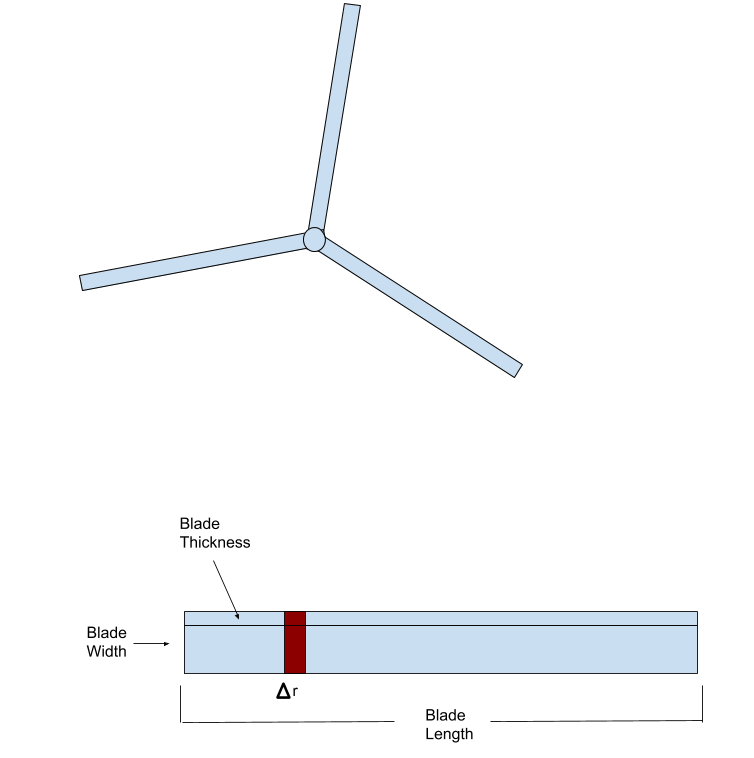
\includegraphics[scale=0.5]{blade}\\
\vspace{0.5\baselineskip} % Whitespace before the editors
$K = \frac{1}{2}\int_{0}^{R}($blade width)(black thickness)(blade density)($\omega r)^2dr$

\pagebreak
\centering % Centre everything on the title page
\vspace{0.5\baselineskip} % Whitespace before the editors
{\LARGE Earth\\} % Title
\vspace{0.5\baselineskip} % Whitespace before the editors
intro goes here\\
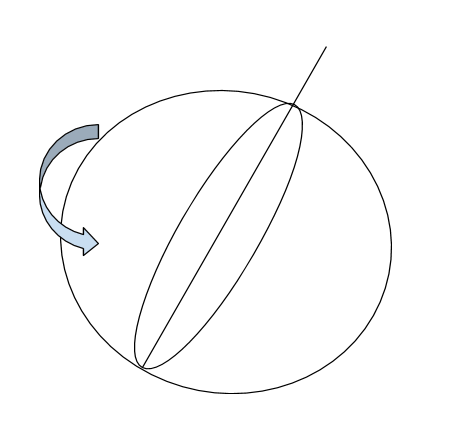
\includegraphics[scale=0.8]{earth}\\
\vspace{0.5\baselineskip} % Whitespace before the editors
\begin{table}[!h]
\begin{tabular}{lll}
Layer & Density & Thickness \\
Crust & $\frac{2.5 g}{cm^3}$ & 30 km \\
Upper Mantle & $\frac{4 g}{cm^3}$ & 720 km \\
Lower Mantle & $\frac{5.1 gm}{cm^3}$ & 2,171 km \\
Inner Core & $\frac{11.2 gm}{cm^3}$ & 2,259 km \\
Outer Core & $\frac{12.9 gm}{cm^3}$ & 1,221 km
\end{tabular}
\end{table}
$\int_{0}^{R}\pi(\sqrt{r^2+R-r^2})^2dr$
%--------------------------------------------------------------------------------------------------------------------------------------------------------------------------
%--------------------------------------------------------------------------------------------------------------------------------------------------------------------------
%--------------------------------------------------------------------------------------------------------------------------------------------------------------------------
%TODO: HELICOPTER WRITE UP, EARTH WRITE UP, SOURCES PAGE PROPERLY FORMATTED, CHECK FOR ILLEGAL CHARS
%--------------------------------------------------------------------------------------------------------------------------------------------------------------------------
%--------------------------------------------------------------------------------------------------------------------------------------------------------------------------
%--------------------------------------------------------------------------------------------------------------------------------------------------------------------------
%--------------------------------------------------------------------------------------------------------------------------------------------------------------------------
\end{document}
